% !TeX spellcheck = id_ID
\documentclass[a4paper,12pt]{article}
\usepackage[bahasa]{babel}
\usepackage{graphicx}
\usepackage{multirow}
\usepackage{enumitem}
\usepackage{listings}
\usepackage{wrapfig}
\usepackage[T1]{fontenc}
\usepackage{inconsolata}
\usepackage{lipsum}
\usepackage{adjustbox}


\usepackage{color}
\usepackage[table]{xcolor}
\definecolor{pblue}{rgb}{0.13,0.13,1}
\definecolor{pgreen}{rgb}{0,0.5,0}
\definecolor{pred}{rgb}{0.9,0,0}
\definecolor{pgrey}{rgb}{0.46,0.45,0.48}
\lstset{language=Java,
	showspaces=false,
	showtabs=false,
	breaklines=true,
	showstringspaces=false,
	breakatwhitespace=true,
	commentstyle=\color{pgreen},
	keywordstyle=\color{pblue},
	stringstyle=\color{pred},
	rulecolor=\color{black},
	basicstyle=\ttfamily,
	moredelim=[il][\textcolor{pgrey}]{$$},
	moredelim=[is][\textcolor{pgrey}]{\%\%}{\%\%}
}

\graphicspath{ {./img/} }
\begin{document}
\title{ {\Large Laporan Praktikum}\\ Algoritma dan Pemrograman \\{\Large Pertemuan 12}}

\author{Aldzikri Dwijayanto Prathama 
	\\195410189
	\\Teknik Informatika}
\makeatletter
\begin{titlepage}
	\begin{center}
		{\huge \bfseries \@title }\\[14ex]
		
\includegraphics[scale=.8]{logo}\\[4ex]
		{\large \@author}\\[19ex]
		{\large \bfseries {SEKOLAH TINGGI MANAJEMEN INFORMATIKA DAN KOMPUTER
				AKAKOM YOGYAKARTA}}
	\end{center}


%{\large \@date} 
\end{titlepage}
\makeatother
%\maketitle
\newpage
\tableofcontents
\newpage

\section{Tujuan}
Mahasiswa dapat mengimplementasikan konsep perulangan while untuk menyelesaikan kasus

\section{Dasar Teori}
\paragraph{}
Pada dasarnya sebuah program dieksekusi secara runtut dari mulai statement yang
pertama kali dibaca dilanjutkan dengan statement yang dibaca berikutnya.
Tetapi alur pemrosesan itu bisa diubah dengan menggunakan seleksi dan
perulangan sehingga memungkinkan sebuah program menjalankan tugas yang lebih
kompleks.
Alur pemrosesan dimulai dari bagian utama program.
\begin{itemize}[label=*.] 
    \item Seleksi dan iterasi/perulangan dapat digabungan dengan dua kemungkinan,
    yang pertama seleksi dalam perulangan dan yang kedua adalah perulangan
    dalam seleksi (akan dibahas pada pertemuan ke-13), gambaran sederhana dari
    model yang pertama adalah:
    \begin{lstlisting}[frame=single]
        for(ungkapan1;ungkapan2;ungkapan3)
        {
            if(kondisi)
            {
                Statement;
            }
        }
    \end{lstlisting}
\end{itemize}
Keterangan
\begin{itemize}[label=*.]
    \item Dalam model ini, statement baru akan dijalankan jika kondisi dalam if bernilai
benar. Statement akan terus dijalankan selama ungkapan2 dalam for masih
bernilai benar.
\end{itemize}
\newpage
\section{Praktik}
\subsection{Praktik 1}
Ketik dan amati hasil output dari program berikut ini\\
\begin{center}
    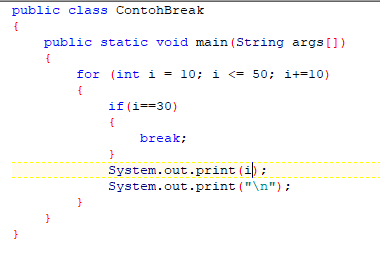
\includegraphics[scale=1]{image1}
\end{center}
Pada program di atas 

\end{document}
